\label{chapt:standards}

Before any complex analysis is completed, initial existing codes and standards will be investigated.\\


The most important parameter in question is the outer diameter $D_o$. For this entire report, it will be assumed that this value is constant at $D_o = 711\ mm = 28\ in$. Based on this fixed parameter, the following relevant values which will be used in this report are summarized below in Table~\ref{table:prelim_params}. All material properties selected as per John Umina's  suggestion from Table 1A of \citep{ASMEbvpcIID} for a SA-106 Grade B steel (most commonly used in seamless pipe). Units shown in both metric (SI) and United States customary (USC).\\

\begin{table}[ht]
	\caption{Key drum parameters and material properties.}
	\centering
%	\begin{tabular}{c c c c}
%		%heading
%		\hline \textbf{Description} & \textbf{Symbol} & \textbf{Value} & \textbf{Units}\\[1 ex]
%		\hline
%		%Main table body content	
%		Outer diameter		&$D_o$			& $28$		& $in$ 	\\
%		Tether diameter		&$D_{thr}$		& $0.6$		& $in$ 	\\
%		Drum length			&$L$			& $49$		& $in$ 	\\
%		Tether tension		&$T$			& $11,525$	& $lbf$	\\	
%		Yield strength		&$S_y$			& $35,000$	& $psi$	\\	
%		Young's Modulus		&$E$			& $2.9\cdot 10^7$ &$psi$\\
%		Poisson's ratio		&$\nu$			& $0.3$		& $ul$	\\	
%		\hline
%	\end{tabular}
    \begin{tabular}{lccccc}
          &       & \multicolumn{2}{c}{\textbf{SI}} & \multicolumn{2}{c}{\textbf{UCS}} \\
	\cmidrule{3-6}    \textbf{Description} & \textbf{Symbol} & \textbf{Value} & \textbf{Units} & \textbf{Value} & \textbf{Units} \\
    \midrule
    Outer diameter & $D_o$ & $711.2$ & $mm$  & $28$ & $in$ \\
    Tether diameter & $D_{thr}$ & $15.2$ & $mm$  & $0.598$ & $in$ \\
    Drum length & $L$   & $1,244.6$ & $mm$  & $49$ & $in$ \\
    Tether tension & $T$   & $51,264$ & $N$   & $11,525$ & $lbf$ \\
    Yield strength & $S_y$ & $241.3$ & $MPa$ & $35,000$ & $psi$ \\
    Young's modulus & $E$   & $200$ & $GPa$ & $2.9\cdot 10^7$ & $psi$ \\
    Poisson's ratio & $\nu$ & $0.3$ & $ul$  & $-$    & $-$ \\
    \end{tabular}%
  \label{table:prelim_params}
\end{table}

Using the above mentioned parameters, as per John Umina's suggestion, the following standards and codes will be investigated.
\begin{itemize}
    \item American Society of Mechanical Engineers (ASME):
	    \begin{itemize}[label=$\bullet$]
	    	\item Boiler and Pressure Vessel Code, Section VIII, Division 1, 2015 \citep{ASMEbvpcVII1}
	    	\item Boiler and Pressure Vessel Code, Section VIII, Division 2, 2015 \citep{ASMEbvpcVII2}
	    \end{itemize}
    \item European Standard EN
        \begin{itemize}[label=$\bullet$]
	       	\item EN 13445-3:2014 \citep{EN134453}
	    \end{itemize}
	\item Det Norske Veritas(DNV) \citep{DNVOSD101}
		    \begin{itemize}[label=$\bullet$]
	    	\item DNV-OS-D101, Marine and Machinery Systems and Equipment\citep{ASMEbvpcVII1}
	    \end{itemize}
	\item Simple hoop stress \citep{roarks}	
\end{itemize}


%----------------------------------------------------------------------------------------------------------------------
\section{Capstan Equation}
What the results in the previous section reveal is that the solution lies in the added level of complexity in this problem. It is required to understand how one wrap of tether in tension results in an external pressure q applied to the outer surface of the cylinder.\\

After much research into this problem, the solution reveals itself into the derivation of the well-known Capstan equation \ref{eq:Capstan}.

\begin{equation}
	\label{eq:Capstan}
	T_2 = T_1 e^{-\mu\theta}
\end{equation}


From this equation, the free body diagram that leads to this solution is presented below in Figure~\ref{fig:Capstan}. 

\begin{figure}[!htbp]
	\centering
	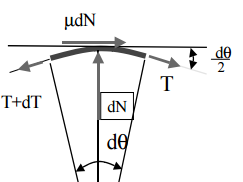
\includegraphics[width=0.6\textwidth]{Capstan}
	\caption{Free body diagram of differential capstan problem.}
	\label{fig:Capstan}
\end{figure}

Based on this, what is of question is how to extrapolate a pressure $q$ from the applied tension $T$. This can be done performing a force balance in the radial direction which reduces to Equation~\ref{eq:CapstanSigRad}.

\begin{equation}
	\label{eq:CapstanSigRad}
	dN-(T+dT)\sin \frac{d\theta}{2}+T\sin \frac{d\theta}{2}= 0
\end{equation}

By assuming a small chance in angle, the substitution of $\sin \theta \approx \theta$ can be made. Applying this relation to \ref{eq:CapstanSigRad} leaves \ref{eq:diffNormal}.

\begin{equation}
	\label{eq:diffNormal}
	dN = T d\theta
\end{equation}

From the above equation, it is now clear that the overall normal force caused by the tension in the cable $T$ can be solved for by integration or as follows \ref{eq:CapstanNorm}

\begin{equation}
	\int_0^N dN =\int_0^{2\pi} T d\theta
\end{equation}

\begin{equation}
	\label{eq:CapstanNorm}
	N=2\pi T	
\end{equation}

With this resultant normal force over one revolution of tether, it is now apparent that the pressure is simply \ref{eq:2_preq}

\begin{equation}
	\label{eq:2_preq}
	p=\frac{N}{A}=\frac{2\pi T}{d\pi D}=\frac{2T}{Dd}
\end{equation}

Using the values from Table~\ref{table:prelim_params} and \ref{eq:2_preq}, $p=1376\  psi\ = 9.484\  MPa$. 

%%----------------------------------------------------------------------------------------------------------------------
\section{ASME's BPVC}

\subsection{Section VIII: Division 1}
As per UG-28 of \citep{ASMEbvpcVII1}, the following procedure was used to calculate the required thickness.
The following list of steps were carried out as per \citep{ASMEbvpcVII1}.

\begin{enumerate}
	\item Assume initial thickness value of $t$
	\item Calculate $D_o/t$ ratio and assure $D_o/t \geq 10$.
	\item Calculate $L/D_o$ ratio, if $L/D_o \geq 50 \Rightarrow 50$ or  $L/D_o \leq 0.05 \Rightarrow 0.05$
	\item With above ratios, go to Figure G of \citep{ASMEbvpcIID} and get value for $A$
	\item With $A$ from above go to chart CS-2 $\because S_y \geq 30 \ ksi$ to get $B$
	\item Using $B$ use Equation \ref{eq:2_VII1_pa} to calculate allowable pressure $p_a$:
		\begin{equation}
			\label{eq:2_VII1_pa}
			p_a = \frac{4B}{3 \left(\frac{D_o}{t} \right)}
		\end{equation}
	\item Check if $p_a \geq p_{req}$ as calculated from \ref{eq:2_preq}, if not, increase $t$ and go to Step 1\\
	
\end{enumerate}

With the Python Script in Appendix A the convergence plot from Figure~\ref{fig:2_vii1_cnvg} below was created.
\begin{figure}[H]
    \centering
    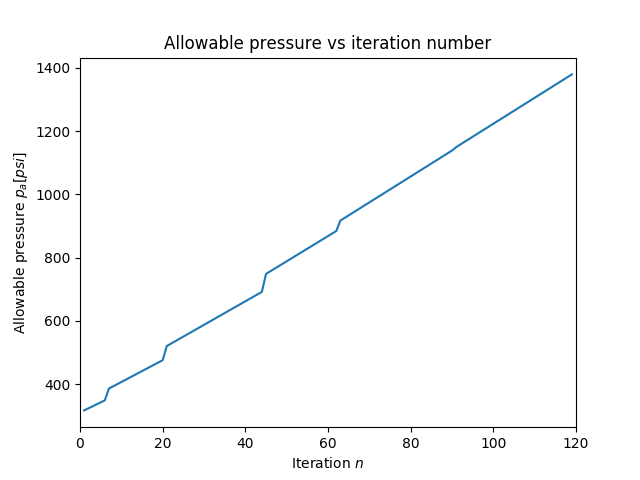
\includegraphics[scale=0.8]{2_vii1_cnvg}
    \caption{Convergence plot of $p_a$.}
    \label{fig:2_vii1_cnvg}
\end{figure}

The script converged at thickness of $t = 43.7\ mm = 1.68\ in$ and an allowable pressure of $p_a\geq p_{req}$ after $n=119$ iterations. 


\subsection{Section VIII: Division 2}
As per subsection 4.4.5 of \citep{ASMEbvpcVII2}, the following procedure was used to calculate the required thickness. Note that only the main formulas will be presented. For intermediate steps, see  Appendix A for Python script utilized during iteration.The following list of steps were carried out as per \citep{ASMEbvpcVII2}.

\begin{enumerate}
	\item Assume initial thickness value of $t$
	\item Calculate elastic buckling stress $F_{he}$ with \ref{eq:2_VII2_4419}
		\begin{equation}
			\label{eq:2_VII2_4419}
			F_{he} = \frac{1.6\ C_h E_y t}{D_o}
		\end{equation}
	\item Based on $S_y$ and $F_{he}$, calculate the predicted buckling stress $F_{ic}$
	\item With subsection 4.4.2 of \citep{ASMEbvpcVII2}, compute the design factor $FS$
	\item Calculate allowable pressure $p_a$ with \ref{eq:2_VII2_4428}
		\begin{equation}
			\label{eq:2_VII2_4428}
			p_a = 2 F_{ha} \left(\frac{t}{D_o}\right)
		\end{equation}
	\item Check if $p_a \geq p_{req}$ as calculated from \ref{eq:2_preq}, if not, increase $t$ and go to Step 1 \\
	
\end{enumerate}

With the Python Script in Appendix A, the convergence plot from Figure~\ref{fig:2_vii2_cnvg} on page~\pageref{fig:2_vii2_cnvg} was created.
\begin{figure}[H]
    \centering
    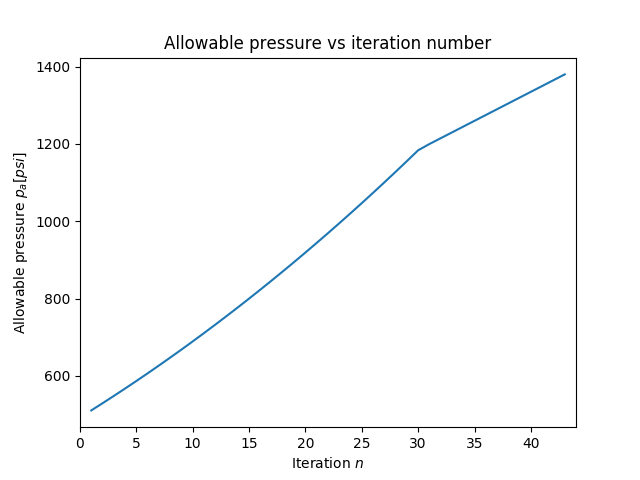
\includegraphics[scale=0.8]{2_vii2_cnvg}
    \caption{Convergence plot of $p_a$.}
    \label{fig:2_vii2_cnvg}
\end{figure}

The script converged at thickness of $t = 23.4\ mm = 0.920\ in$ and an allowable pressure of $p_a\geq p_{req}$ after $n=43$ iterations. 


%%----------------------------------------------------------------------------------------------------------------------
\section{European Standard}
\subsection{EN-13445-3}
As per subsection 8.5.2.2 of \citep{EN134453}, the following procedure was used to calculate the required thickness $e_a$.

\begin{enumerate}
	\item Assume initial thickness value of $e_a$ and calculate $p_y$ with \ref{eq:2_EN_py}
		\begin{equation}
			\label{eq:2_EN_py}
			p_y = \frac{\sigma_e e_a}{R}
		\end{equation}
	\item Compute the lower failure pressure $p_m$ \ref{eq:2_EN_pm}, see 8.5.2.6 of \citep{EN134453} for $\varepsilon$
		\begin{equation}
			\label{eq:2_EN_pm}
			p_m = \frac{E e_a  \varepsilon}{R}
		\end{equation}
	\item With the $p_m/p_y$ ratio, use Figure 8.5.5 of \citep{EN134453} to find equivalent $p_r/p_y$
	\item Rearrange for $p_r$ and calculate allowable pressure $p$ ith \ref{eq:2_EN_pa}
		\begin{equation}
			\label{eq:2_EN_pa}
			p = \frac{p_r}{S}
		\end{equation}
	\item Check if $p \geq p_{req}$ as calculated from \ref{eq:2_preq}, if not, increase $e_a$ and go to Step 1 \\
\end{enumerate}

With the Python Script from Appendix A the convergence plot from Figure~\ref{fig:2_en13445_cnvg}.
\begin{figure}[H]
    \centering
    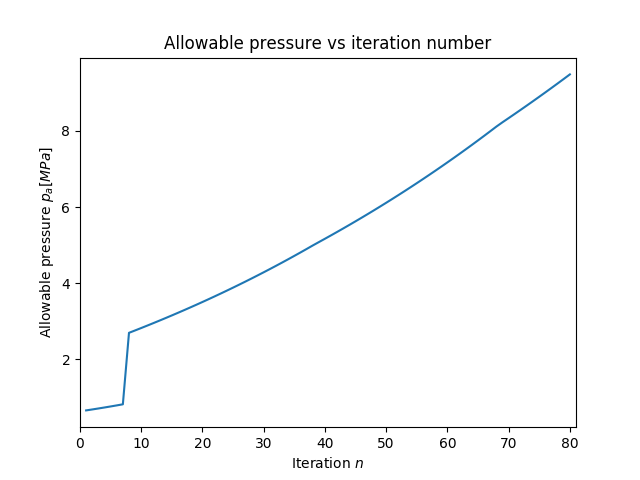
\includegraphics[scale=0.8]{2_en13445_cnvg}
    \caption{Convergence plot of $p_a$.}
    \label{fig:2_en13445_cnvg}
\end{figure}

The script converged at thickness of $e_a = 32.8\ mm = 1.290\ in$ and an allowable pressure of $p\geq p_{req}$ after $n=80$ iterations. 
\pagebreak

%%----------------------------------------------------------------------------------------------------------------------
\section{DNV}

\subsection{DNV-OS-D101}

As per \citep{DNVOSD101}, in subsection F215, Equation~\ref{eq:2_DNV_hoop} is presented as follows.

\begin{equation}
	\label{eq:2_DNV_hoop}
	\sigma_h = C\cdot\frac{T}{d_{thr}t}
\end{equation}

In this equation, $C$ is a factor based on the number of wraps on the drum,. for two layers $C=1.75$. It is also to be noted that the hoop stress is limited to $\sigma_h \leq 0.85\cdot S_y$. \\

For this application, rearranging for $t$, setting $\sigma_h = S_{allow}=S_y/SF$ (see Table~\ref{table:prelim_params})and solving accordingly will yield a valid value of $t = 36.6\ mm = 1.440 \ in$. 

%----------------------------------------------------------------------------------------------------------------------
\section{Hoop Stress}

Using the well known hoop stress equation \citep{roarks} for a thin walled pressure vessel (TWPV), Equation~\ref{eq:2_hoop} is presented as follows.

\begin{equation}
	\label{eq:2_hoop}
	\sigma_h = \frac{pR}{t}
\end{equation}

Again, rearranging for $t$ and setting $\sigma_h = S_{allow}=S_y/SF$, solving accordingly will yield a valid value of $t = 21.0\ mm = 0.825 \ in$. Note that $\because R/t = 17 \geq 10$, the assumption of a TWPV is valid.

\pagebreak

%%----------------------------------------------------------------------------------------------------------------------
\section{Comparison}

Based on the above sections, the results are summarized in Table~\ref{table:2_comp}.
\begin{table}[htbp]
  \centering
  \caption{Comparison $t$ according to method used.}
    \begin{tabular}{lccc}
          & \multicolumn{2}{c}{\textbf{Results}} &  \\
    \textbf{Method} & \textbf{mm} & \textbf{in} & \textbf{SF} \\
    \midrule
    ASME BPVC VII-1 & $43.7$  & $1.680$ & $1.5$ \\
    ASME BPVC VII-2 & $23.4$  & $0.920$ & $1.5$ \\
    EN 13445-3 & $32.8$  & $1.290$ & $1.5$ \\    
    DNV-OS-D101 & $36.6$  & $1.440$ & $1.5$ \\
    Hoop	& $21.0$ &$0.825$ & $1.5$\\
    \end{tabular}%
  \label{table:2_comp}%
\end{table}%

